% Opciones empleadas:
%
%	a4paper -> indica el tamaño del papel, en este caso A4.
%	11pt -> tamaño de la fuente 11 puntos.
%	oneside -> sólo escribimos en una cara del folio.
% 
% Otras opciones interesantes:
%
%	twoside -> escribimos a doble cara.
%	openbib -> para que las referencias bibliográficas tengan un salto de línea entre cada campo de la referencia.
%
\documentclass[a4paper,11pt,twoside]{book}

% configuración de márgenes
\usepackage{setspace}
\doublespacing
\setlength\textwidth{15cm}
\setlength\textheight{22cm}
\setlength\oddsidemargin{1cm}
\setlength\evensidemargin{0cm}

% codificación utf8x y símbolos del idioma español (ñ, acentos, ...)
% el documento será necesario editarlo en utf-8
\usepackage[english]{babel}
\usepackage[utf8x]{inputenc}
\usepackage{morefloats}

% puede que queramos usar el símbolo del euro.
\usepackage{eurosym}

% El paquete fancybox nos permite crear cajas de diferentes estilos con facilidad.
% http://www.ctan.org/get/macros/latex/contrib/fancybox/fancybox.pdf
% http://www.mackichan.com/index.html?techtalk/487.htm~mainFrame
\usepackage{fancybox}
\usepackage{multicol}
\usepackage{amsmath}

% Para incluir subfiguras.
\usepackage{subfigure}

% Para incluir gráficos en JPG => compilar con pdflatex.
%\usepackage[pdftex]{graphicx}

% Para incluir gráficos EPS => compilar con latex.
\usepackage[dvips]{graphicx}
%\graphicspath{ {Graphics/} }

% Para escribir en color...
%
% ... cuando compilamos con el comando ``latex''
\usepackage[dvips,usenames]{color}
% ... uando compilamos con el comando ``pdflatex''
% \usepackage[pdftex,usenames,dvipsnames]{color}

% Para realiza hiperenlaces
\usepackage[pagebackref=true]{hyperref}
\hypersetup{
    bookmarks=true,         % barra de marcadores
    unicode=false,          % caracteres non-Latin en marcadores de Acrobat
    pdftoolbar=true,        % mostrar barra de herramientas de Acrobat
    pdfmenubar=true,        % mostrar menú de Acrobat
    pdffitwindow=false,     % ajustar ventana al ancho de página
    pdfstartview={FitH},    % ajustar documento al ancho de página
    pdftitle={Memoria BIBEM},    % título
    pdfauthor={},     % autor
    pdfsubject={},   % tema del documento
    pdfcreator={},   % generador del documento
    pdfproducer={}, % productor del documento
    pdfkeywords={}, % lista de palabras clave
    pdfnewwindow=true,      % enlaces en una nueva ventana
    colorlinks=true,       % false: enlaces en caja; true: enlaces coloreados
    linkcolor=blue,          % color de enlaces internos
    citecolor=green,        % color de enlaces a bibliografía
    filecolor=magenta,      % color de enlaces a ficheros
    urlcolor=blue           % color de enlaces externos
}

% Espaciado y ajuste de márgenes
\usepackage{setspace}
\onehalfspacing
% \doublespacing
\setlength{\textwidth}{15cm}
\setlength{\textheight}{22cm}

% Para evitar lineas huérfanas
\widowpenalty=10000
\clubpenalty=10000

% Paquete fancyhdr -> Para modificar la cabecera y pie de páginas.
% http://tug.ctan.org/tex-archive/macros/latex/contrib/fancyhdr/
\usepackage{fancyhdr}
\pagestyle{fancy}
\fancyhf{}
\fancyhf[HR]{\thepage}
\fancyhf[HL]{\nouppercase\rightmark}

% Package booktabs -> Para mejorar el aspecto de las tablas o cuadros.
% http://www.ctan.org/tex-archive/macros/latex/contrib/booktabs/
\usepackage{booktabs}

% Package rotating -> Para poder girar las tablas y dibujarlas a lo largo
% del folio en vez de a lo ancho.
\usepackage{rotating}

% Packages multicol y multirow, para manejar tablas de filas y columnas múltiples.
\usepackage{multicol}
\usepackage{multirow}

% Para empotrar código con resaltado
\usepackage{listings, color}
%Ahora toca configurar el entorno para el código fuente
\definecolor{gray97}{gray}{.97}
\definecolor{gray75}{gray}{.75}
\definecolor{gray45}{gray}{.45}

\lstset{ frame=Ltb,
     framerule=0pt,
     aboveskip=0.5cm,
     framextopmargin=3pt,
     framexbottommargin=3pt,
     framexleftmargin=0.4cm,
     framesep=0pt,
     rulesep=.4pt,
     backgroundcolor=\color{gray97},
     rulesepcolor=\color{black},
     %
     stringstyle=\ttfamily,
     showstringspaces = false,
     basicstyle=\small\ttfamily,
     commentstyle=\color{gray45},
     keywordstyle=\bfseries,
     %
     numbers=left,
     numbersep=15pt,
     numberstyle=\tiny,
     numberfirstline = false,
     breaklines=true,
   }

% minimizar fragmentado de listados
\lstnewenvironment{listing}[1][]
   {\lstset{#1}\pagebreak[0]}{\pagebreak[0]}

\lstdefinestyle{consola}
   {basicstyle=\scriptsize\bf\ttfamily,
    backgroundcolor=\color{gray75},
   }

\lstdefinestyle{SQL}
   {language=SQL,
   }

\lstdefinestyle{Java}
   {language=Java,
   }

\usepackage{url}


% Personalizamos la separación entre párrafos...
\parskip=6pt

% Personalizamos el identado en la primera línea del nuevo párrafo...
\parindent=10pt

% Establecemos el número máximo de niveles de profundidad en las secciones.
\setcounter{secnumdepth}{3}

% Título
\title{Solving the magic square problem with the NSGA II genetic algorithm}
% Autor
\author{Petra Franjic \and Gustavo Puig}
% Fecha
\date{\today}


\begin{document}

	% \maketitle sirve para generar automática una portada predefinida, pero para un proyecto fin de carrera
	%	de FIC no sirviría porque no cumple las normas de presentación. Podemos hacer dos cosas:
	% 1. Usarla e ignorar las normas (y asumir las consecuencias que pueda tener)
	% 2. Hacernos una portada en LaTeX que cumpla las normas (menos arriesgado)
	%
        %
% Portada.
%

% Nota: Será más cómodo emplear el comando \maketitle que genera una portada de forma automática, pero 
% no incluye toda la información que es necesario incluir en la memoria de un proyecto de fin de carrera
% de la Facultad de Informática de A Coruña.
%

\graphicspath{ {Graphics/} }

\begin{titlepage}

	\begin{center}

		% Logotipo de la universidad.
		%
\includegraphics[width = 6cm] {logocei.pdf}
		\vspace{2cm}

		% Nombre de la facultad, de la universidad y del departamento en que se realiza el PFC.
		{\Large{\textbf{UNIVERSITY OF INFORMATICS OF MADRID - UPM}}}
		\\
		{\it \large{\textbf{ARTIFICIAL INTELLIGENCE DEPARMENT}}}
		\vspace{1cm}

		% Indicamos el nombre de la titulación oficial que hemos cursado con tanto esfuerzo.
		{\large INTELLIGENT SERCHING BASED ON METHAHEURISTICS\\MASTER IN ARTIFICIAL INTELLIGENCE}
		\vspace{1cm}

		% Título
		\textbf{\Large Genetic Algorithms}
		\vspace{7cm}
	\end{center}

	\begin{flushright}
		\begin{tabular}{ll}
			% Nombre del alumno.
			\large{\textbf{Alumni:}}	&
			\large{Petra Franjic, Gustavo Puig} \\

			% Nombre del director/tutor del proyecto.
			\large{\textbf{Professor:}}	&
			\large{Director que corresponda} \\

			% Fecha.
			\large{\textbf{Date:}}	&
			\large{2th November 2015} \\
		\end{tabular}
	\end{flushright}

\end{titlepage}

        
        \newpage
	$\ $
	\thispagestyle{empty} % para que no se numere esta pagina

	% Los proyectos de fin de carrera de FIC han de ir acompañados de una serie de documentos adicionales, algunos
	% 	de ellos obligatorios (certificado, resumen, lista de palabras clave) y otros opcionales (dedicatoria
	%	y agradecimientos).
	%
	\setcounter{page}{1}
        %
% Resumen del proyecto de fin de carrera
%

\section*{Abstract:}

The aim of this practical assignment was to implement and analyze a multi-objective genetic algorithm with the goal of obtaining the solution of the magic square problem, which is a combinatorial optimization problem. The algorithm that was chosen for this task is the Non-dominated Sorting Genetic Algorithm II (NSGA-II). Simulations with different parameter values were conducted and the performance of the algorithm was measured. The first part of the documentation explains different aspects of the workings of the algorithm and in the second part the results of the carried out simulations are presented and discussed.
        %%
% Palabras clave
%

\section*{Key words List:}

List separated by commas


        %%
% Dedicatoria
%
\chapter*{}

\begin{flushright}
	{\it Knight Rider, a shadowy flight into the dangerous world of a man who does not exist. Michael Knight, a young loner on a crusade to champion the cause of the innocent, the helpless in a world of criminals who operate above the law.}
\end{flushright}

        %%
% Agradecimientos
%

\chapter*{Gratitudes\footnote{In alphabetic order}}

A D. Profesor que corresponda (Posición del profesor), agradecimiento que se quiera poner.



	% FRONTMATTER: TOC, LOF, LOT y descripción/organización de la memoria.
        \frontmatter

%%% DELETED - INCLUDE IF IT'S NECESSARY
        \tableofcontents
        %\listoffigures
        %\listoftables

        %
% Frontmatter - Introducción. Los miembros del tribunal que juzgan los PFC's tienen muchas más memorias que leer, por lo que
%	agradecerán cualquier detalle que permita facilitarles la vida. En este sentido, realizar una pequeña introducción,
%	comentar la organización y estructura de la memoria y resumir brevemente cada capítulo puede ser una buena práctica
%	que permita al lector centrarse fácilmente en la parte que más le interesa.
%

\chapter[Introduccion]{
	Introduccion
}
Genetic algorithms (GAs) belong to a family of stochastic search methods which is covered by the generic term Evolutionary Computation (EC). The main characteristic of EC techniques is that they computationally simulate the natural evolutionary process. The evolutionary process is modeled by the neo-Darwinian paradigm, which combines Darwinian evolution with Mendelian genetics. Other techniques covered by EC are evolution strategies (ESs) and evolutionary programming (EP).
The EC family of optimization techniques finds its place among other stochastic search and optimization approaches such as Simulated Annealing, Monte Carlo methods and Tabu search. These stochastic approaches were developed as an alternative to solving high-dimensional, discontinuous and multimodal problems, where traditional deterministic search techniques often proved ineffective. The disadvantage of these methods is that they don't guarantee to find the absolute best solution, but they do promise to find an acceptable solution in a reasonable amount of time.
A chromosome or an individual is an encoded candidate solution to a problem. It corresponds to a biological genotype. Chromosomes are typically represented as strings of some predefined alphabet A. The alphabet can be binary or non-binary. Typical examples of non-binary alphabets are real and integer numbers. The phenotype of an individual is the point in the solution space that this individual genotype maps to. A population is a set of individuals. Genes encode a particular element of the candidate solution. The values which a gene can take are called alleles.
***Figure search space solution space***
All evolutionary algorithms share a number of common properties. Firstly, all of them utilize the collective learning process of a population of individuals. Secondly, descendants of individuals are generated by randomized processes intended to model mutation and recombination occurring in nature. Lastly, by means of evaluating individuals in their environment, all individuals are assigned a measure of quality or fitness. This way, it is possible to make a comparison of individual fitness. This is the basis of the process of selection, which favors better individuals to reproduce more often than those relatively worse.
There are several basic differences in the utilization of these principles which make genetic algorithms different from the rest of the techniques of EC. Genetic algorithms emphasize recombination (crossover) as the most important search operator and apply mutation with a very small probability. They also use a probabilistic selection operator and often rely on the binary representation of individuals.
The general principle by which the genetic algorithm works is as follows. There exists a population of individuals where each individual represents one possible solution to the given problem. Each individual can be assigned a fitness measure by calculating the value of the function that is being optimized. The selection operator is used to choose those individuals in the population which are going to become the parents of the next generation. The parents produce children by means of the crossover operator, which emulates genetic recombination. Next the mutation operator is applied on the children. Lastly, the reinsertion operator is used to include children in the population of solutions, which closes the cycle of an algorithm.

Algorithm

General algorithm design
There are two typical genetic algorithm designs, the steady-state genetic algorithm and the generational genetic algorithm.
The steady-state genetic algorithm or incremental algorithm can be thought of as a simpler version of the generational genetic algorithm. At every cycle of the algorithm, two parents are chosen, the crossover operator is applied and a child is formed. The child is subsequently mutated and inserted in the population. Since the population size is maintained constant, the child replaces an individual in the old generation. The individual to be replaced is typically the worst one in the population.
Contrary to the steady-state genetic algorithm, the generational genetic algorithm makes a clear distinction between parents and children. At each algorithm cycle, a new generation, composed exclusively of children is formed and the old generation dies out.
In this practical assignment we have chosen to implement the steady-state algorithm with replacement of the worst individual in the population. The main reason against the generational approach is that absence of elitism would have made the convergence process slower. An additional reason for choosing the steady-state algorithm is the much lower computational cost needed to generate each generation of individuals. The scheme of the algorithm is shown in Figure ? and the pseudocode is shown in figure ?.
*** The scheme of the algorithm ***
*** The pseudocode of the algorithm ***


I'll have to add some modifications to the implementation so that the new generation is formed by choosing best individuals in the set of parents + children


Implementation
Class diagrams + explanations + code


Bibliography:
Redes de neuronas artificiales y computacion evolutiva
EAMOP
handbook of CE
Cupic(home university book)

%
% SECCION
%
%\subsection*{Estructura de la memoria}
%
%\paragraph*{Capítulo 1.}
%Resumen capítulo
%
%\paragraph*{Capítulo 2.}
%Resumen capítulo
%
%\paragraph*{Capítulo 3.}
%Resumen capítulo
%
%\paragraph*{Capítulo 4.}
%Resumen capítulo
%
%\paragraph*{Capítulo 5.}
%Resumen capítulo
%
%\paragraph*{Capítulo 6.}
%Resumen capítulo
%
%\paragraph*{Capítulo 7.}
%Resumen capítulo
%
%\paragraph*{Capítulo 8.}
%Resumen capítulo
%
%\paragraph*{Capítulo 9.}
%Resumen capítulo
%
%\paragraph*{Capítulo 10.}
Resumen capítulo


	% MAINMATTER: El contenido, capítulo a capítulo, de la memoria del PFC.
        \mainmatter

	\providecommand{\abs}[1]{\lvert#1\rvert}

\chapter[Problem design]{\label{identificadorReferenciaCruzada}
Problem design}

\ \ To use NSGA-II to solve the problem of the magic square, it was required to set up the magic square problem as a constraint satisfaction multi-objective problem. We imposed two constraints on the problem and 9 optimization goals which followed proposed solutions for similar problems, like Sudoku puzzle solving [7].

By the nature of the magic square each number between 1 and $n^2$ has to appear in the square exactly once. This rule was imposed with the two mentioned constraints. The  first constraint maintained that the sum of all of the numbers in the square is equal to $0.5 * n^2 * (n^2 + 1)$, or, in the particular case of a $4 x 4$ magic square, to the sum of all numbers from 1 to 16. The second constraint maintained that the product of all numbers in the square equals to $(n^2)!$, or in the particular case of a $4 x 4$ magic square, to $16!$. The constraints in algebraic form:

\begin{equation}
\frac{n^{2}(n^{2} +1)}{2} - \sum_{i}^n \sum_{j}^n x_{i,j} = 0
\end{equation}

\begin{equation}
(n^2)! - \prod_{i}^{n} \prod_{j}^{n} x_{i,j} = 0
\end{equation}

To guide the algorithm towards optimal solutions, it was necessary to use additional knowledge about the problem. The additional knowledge that we took into account was that considering a magic square with dimension n, the sum in each of the sub-blocks (rows, columns, diagonal) equals $0.5 * n * (n^2 + 1)$ [8]. This consideration was necessary because only those sub-blocks which sum to this value can contribute to an optimal solution. It is not enough, for an example, to consider as better those solutions for which can be said only that they have more of these sub- blocks summing to the same value. The functions that were being minimized in algebraic form:

\begin{equation}
f_{1}(x) = \abs{\frac{n(n^2+1)}{2}-\sum_{j}^n x_{1,j}}
\end{equation}
\begin{center}
...
\end{center}
\begin{equation}
f_{5}(x) = \abs{\frac{n(n^2+1)}{2}-\sum_{i}^n x_{i,1}}
\end{equation}
\begin{center}
...
\end{center}
\begin{equation}
f_{9}(x) = \abs{\frac{n(n^2+1)}{2}-\sum_{i}^n x_{i,j}}
\end{equation}


	\chapter[NSGA-II algorithm]{\label{identificadorReferenciaCruzada}
NSGA-II algorithm}


	\section[Outline of genetic algorithms]{\label{identificadorReferenciaCruzada}
Outline of genetic algorithms}

	\section[Search components of the NSGA-II algorithm]{\label{identificadorReferenciaCruzada}
Search components of the NSGA-II algorithm}

\ \ In addition to the common concepts of single-objective metaheuristics, a multi-objective metaheuristics has to deal with three additional main search problems. Here these components are identified and in the following sections a detailed explanation will be given of the methods NSGA-II uses to address each of the problems. The first problem is the fitness assignment which has the role of guiding the search algorithm towards Pareto optimal solutions for a better convergence. This procedure assigns a scalar-valued fitness to a vector objective function [5]. NSGA-II employs a dominance based approach for this component of the search algorithm. The second search problem is the preservation of diversity where emphasis is on generating a diverse set of Pareto solutions in the objective space and helping the exploration of the fitness space [2]. The NSGA-II here employs a nearest-neighbor approach through calculating the crowding distance. Lastly, elitism guides the search towards preservation and use of elite solutions which allows a robust, fast, and monotonically improving performance of tje metaheuristic.
	\subsection[Dominance based ranking]{\label{identificadorReferenciaCruzada}
Dominance based ranking}

	\subsection[Crowding distance]{\label{identificadorReferenciaCruzada}
Crowding distance}

\ \ There are several nearest-neighbor approaches that can be employed to evaluate the distribution of solutions and the crowding distance has proved to be one of the more eficient [2]. The crowding distance of a solution is de ned as the circumference of the rectangle de ned by its left and right neighbors, and infinity if there is no neighbor. Figure 2 illustrates the concept of crowding. Solutions with high crowding distance are considered better solutions, as they introduce more diversity in the population. In Figure 1 the solutions a and d belonging to the rank 1 in terms of non-dominance have the best score in terms of crowding. Then follows the solution b and then c. The rectangle associated with c is the smallest one [5]. NSGA-II uses crowding distance in its selection operator to keep a diverse front by making sure each member stays a crowding distance apart.
\begin{figure}[h!]
\begin{center}
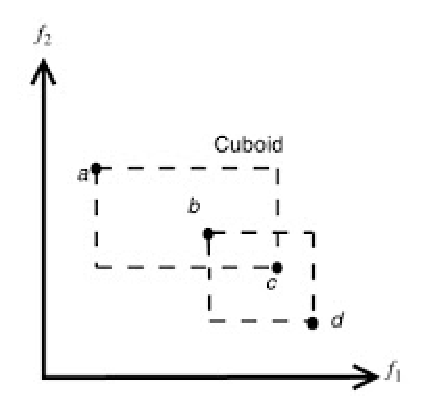
\includegraphics[width = 5cm] {./Graphics/Figure2.eps} 

\caption{Crowding distance [5]}
\end{center}
\end{figure}
	\subsection[Elitism]{\label{identificadorReferenciaCruzada}
Elitism}

\ \ Elitism consists of archiving the best solutions generated during the search. Elitism in NSGA-II is evident in the general outline of the algorithm. The key phase here is the replacement of individuals in the old generation. Before the replacement phase individuals in the old generation are sorted according to their ?goodness? together with the newly generated o spring. This allows the best individuals of the older generation to be passed in the next generation. The mechanism can be seen in Figure 3. P(sub)t is the parents population and Q(sub)t is the o spring population at generation t. F1 are the best solutions from the combined populations (parents and
o spring). F2 are the second best solutions and so on.

\begin{figure}[h!]
\begin{center}
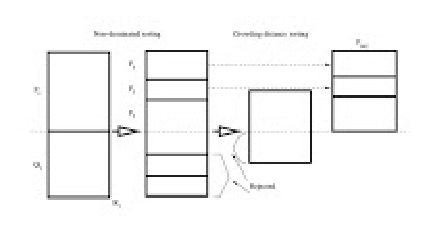
\includegraphics[width = 10cm] {./Graphics/Figure3.eps} 

\caption{Flow diagram that shows the way in which the NSGA-II elitism works.}
\end{center}
\end{figure}
	\section[Outline of the NSGA-II algorithm]{\label{identificadorReferenciaCruzada}
Outline of the NSGA-II algorithm}

	\section[Codification]{\label{identificadorReferenciaCruzada}
Codification}

\ \ Two types of codification can be used to represent points in the solution space, binary and non-binary codification. Generally it can?t be said that one codification is better than the other, as it depends on the problem that is being dealt with.

Considering the design of the assigned problem, we have decided to use non- binary integer codification as the more simple and straightforward of the two possible codification. An additional reason against binary coded solutions was the fact that the magic square is a combinatorial optimization problem, which imposes a set of constraints on the possible solutions. By applying common crossover and mutation operators on bit strings it would be very difficult to respect the given constraint that the numbers should stay in the 1 to $n^2$ range, or that each of the numbers in the square should appear only once.

It is interesting to note the duality in the viewpoint of variables and values for this particular problem as was expressed in [6]. The array of numbers for codifying the square could be considered as either codifying the problem of finding the number to go in each cell of the square, or deciding which cell to put each number in. We have decided to go with the first approach since the constraints on the row and column sums are much easier to express.


	\section[Operators]{\label{identificadorReferenciaCruzada}
Operators}

	\subsection[The crossover operator]{\label{identificadorReferenciaCruzada}
The crossover operator}

\ \ The crossover operator that was used can be described as a larger scale uniform crossover. Two versions of the crossover were used, one that worked by recombining the rows of the parents, and the other that recombined the columns. Each was applied with equal probability. This alternation was necessary because passing on rows or columns from the parents to the children could be equally beneficial.

The workings of the crossover can be described as follows, for the case of rows, and the explanation is analogous for the columns. First a mask of zeros and ones is formed, with the same length as is the number of rows. For each position in the mask, the symbol defines from which parent the row will be taken to form the child. Next a child is generated according to the scheme. For an example, mask 1010 means that the first and third row will be taken from the first parent and the second and fourth row from the second parent. Each of the symbols has an equal probability of being generated which means that the child will inherit approximately half of the rows from the first parent and half from the second.

Although a gene is considered a single position in the square, we have decided against applying the crossover operator on this scale. The reason is that the sub-blocks (rows and columns) are the smallest units where beneficial changes could occur that we would like to get passed on to the children. In other words, if the sum of the numbers in one of the rows is equal to the target value, we wouldn?t want a crossover operator to break the row.

The chosen crossover operator can generate infeasible solutions, where any of the numbers from 1 to $n^2$ is present more than once in the square, and some of them do not appear at all. As was discussed with the design of the problem, these solutions are marked as violating the constraints of the problem and are not further considered.
	\subsection[The mutation operator]{\label{identificadorReferenciaCruzada}
The mutation operator}

	\chapter[Implementation]{\label{identificadorReferenciaCruzada}
Implementation}

	\chapter[Conclusion]{\label{identificadorReferenciaCruzada}
Conclusion}



	\backmatter
	% INCLUIMOS LOS APÉNDICES... !! DELETED - INCLUDE IF IT'S NECESSARY
        %\appendix
	%%
% Memoria económica.
%

\chapter[Título de apéndice]{
	Título de apéndice.
}

Lorem ipsum dolor sit amet, consectetur adipiscing elit. Integer luctus varius augue vel imperdiet. Maecenas neque turpis, accumsan ut eleifend vel, eleifend gravida est. Duis mattis pulvinar porta. Nunc consequat, felis ut malesuada egestas, ipsum urna sodales enim, eu lobortis mauris tellus in augue. In tristique tortor id nisi placerat et rutrum tortor auctor. Aenean erat elit, faucibus non egestas semper, volutpat sit amet ante. Nam nulla justo, suscipit nec sagittis sed, varius id magna. Duis a lorem id felis eleifend aliquet eget vel arcu. Etiam ultricies diam a magna facilisis ornare. Integer tempor massa quis sem gravida bibendum. Sed massa felis, condimentum sit amet bibendum in, tristique sit amet mauris. Nullam tellus ante, ornare eget mollis ac, gravida id nunc. Donec elit neque, aliquam eget auctor sed, gravida in nibh. Vestibulum sit amet diam a magna tempor bibendum quis a ante. Integer augue sapien, facilisis ac malesuada sed, consectetur id turpis. Quisque a leo dapibus felis aliquet vestibulum vitae vitae urna. Nunc ut felis ut metus gravida ultricies. Cras tincidunt nisi ante. Nunc eu quam interdum dui cursus lacinia. Praesent adipiscing ultrices nulla at posuere.

Aliquam gravida facilisis eleifend. Nunc id lorem nibh. Nulla facilisi. Nunc suscipit lectus quis tellus adipiscing adipiscing. Proin ipsum justo, egestas dictum iaculis et, pretium non diam. Aenean vehicula hendrerit lectus, vel bibendum nisi volutpat quis. Fusce molestie condimentum libero, nec scelerisque nisi mollis et. Aliquam placerat accumsan congue. In scelerisque nulla sit amet mauris consectetur consectetur. Suspendisse mattis mi in sapien egestas sit amet accumsan urna sagittis. Mauris metus massa, porta at rutrum eget, sollicitudin eu risus. Donec non diam erat. Nam sagittis, nibh non fermentum ornare, ipsum est mollis felis, eget vulputate tellus ante at erat. Praesent porta tempus velit at faucibus. Donec rhoncus varius nunc, eget imperdiet ligula blandit eget. Morbi pulvinar, nunc ac porta interdum, mauris ligula sollicitudin sem, et sollicitudin turpis magna eu lectus. Pellentesque nulla dui, feugiat quis pharetra eu, accumsan imperdiet quam. Aenean lacinia porttitor leo vitae hendrerit. Pellentesque dictum ultricies dui, et rhoncus nulla sagittis ut. Suspendisse suscipit, risus sed posuere rhoncus, neque metus scelerisque diam, eu gravida quam orci eu dui.

Nulla sit amet sem massa, aliquet auctor magna. Vivamus quis magna sollicitudin felis bibendum mollis. Etiam elementum lacus id quam tincidunt pulvinar. Ut vehicula aliquam ante, vel venenatis libero bibendum eget. Sed gravida lobortis velit, et ornare nunc ullamcorper et. Morbi neque sapien, mattis id semper in, varius at arcu. Duis aliquam ornare sem, eu sagittis libero facilisis non. Nunc quis ultricies augue. Pellentesque ac nulla libero, ut suscipit dui. Morbi aliquet quam non metus iaculis quis accumsan ipsum consectetur.

Mauris mauris odio, varius quis accumsan bibendum, vulputate vel tellus. Sed non consectetur eros. Aenean et mi ut est tincidunt commodo. Donec nunc metus, facilisis a consequat vitae, dignissim quis leo. Cras condimentum, felis a molestie viverra, massa eros consequat nisl, at porta nibh sapien condimentum ante. Duis convallis velit quis metus pulvinar convallis. Suspendisse sed purus non purus dictum ultricies in vitae nisl. Cras convallis erat eu ipsum molestie fermentum. Mauris turpis nunc, condimentum non aliquam ac, ornare at lectus. Donec scelerisque fermentum malesuada. Praesent urna nisl, iaculis sed pharetra eu, tincidunt et lectus. Nulla posuere eros at elit vehicula laoreet. Sed ut erat orci, ac pellentesque nibh. Nulla at sapien sed justo luctus laoreet.

Sed convallis massa laoreet mi venenatis eget dapibus orci varius. Pellentesque purus nisi, placerat nec pretium ac, pretium vitae augue. Vivamus eleifend vestibulum mi, ac dignissim urna vulputate vel. Integer volutpat neque purus. Nulla hendrerit tempus est nec aliquet. Ut facilisis bibendum nisl eget porttitor. Cum sociis natoque penatibus et magnis dis parturient montes, nascetur ridiculus mus. Fusce consectetur sem eget ante rhoncus nec mollis lorem volutpat. Fusce in libero lectus, ut gravida lectus. Nam nulla nunc, dignissim sed sollicitudin a, commodo vel felis. Donec lacinia justo quis neque tempor interdum ut cursus mi. Phasellus venenatis porttitor mi consectetur egestas. Pellentesque quis elit nibh. Pellentesque molestie turpis ac arcu gravida sed ultricies felis pulvinar.

%         \include{pfc_appendix_020}

	
	% INCLUIMOS LA BIBLIOGRAFÍA...
	\nocite{*}	% Se usa para indicar en la bibliografía las referencias no citadas.
	\bibliography{biblio}
	\bibliographystyle{plain}

\end{document}

